\section{Fighting Byzantine Contributions in Heterogeneous Settings}

\begin{frame}
  \sectionpage

  \fcitefootnote{lavaur_radar_2024}
\end{frame}


\begin{frame}{Context}
  % - case study (multiple organizations, partial heterogeneity)
  % - Byzantine contributions -> no guaranties
  \textbf{Case study reminder}
  \begin{itemize}
    \item Multiple organizations collaborating on a federated intrusion detection system.
    \item Partial heterogeneity in the datasets: organizations have different data distributions but can share similarities.
  \end{itemize}

  \textbf{Byzantine contributions}
  \begin{itemize}
    \item No guarantees on the quality of the contributions.
    \item Can be intentional, due to poor data quality, or due to data distribution mismatches.
  \end{itemize}

\end{frame}

\begin{frame}{Problem Statement}
  \begin{block}{Quality Assessment in Heterogeneous Settings}
    For $n$ participants $p_i$ and their local datasets $d_i$ of unknown similarity, each participant uploads a model update $w_i^r$ at each round $r$. Given $P = \{ p_1, p_2, \dots, p_n \} $ and $W = \{ w_1^r, w_2^r, \dots, w_n^r \} $, how can one assess the quality of each participant’s contribution without making assumptions on the data distribution across the datasets $d_i$?
  \end{block}
\end{frame}

\begin{frame}{Existing Solutions}

  \begin{columns}[T]
    
    \begin{column}{.33\textwidth}
      \small\centering
      \textbf{Server-side evaluation}~\autocite{zhou_DifferentiallyPrivateFederated_2022}

      \begin{figure}
        \centering
        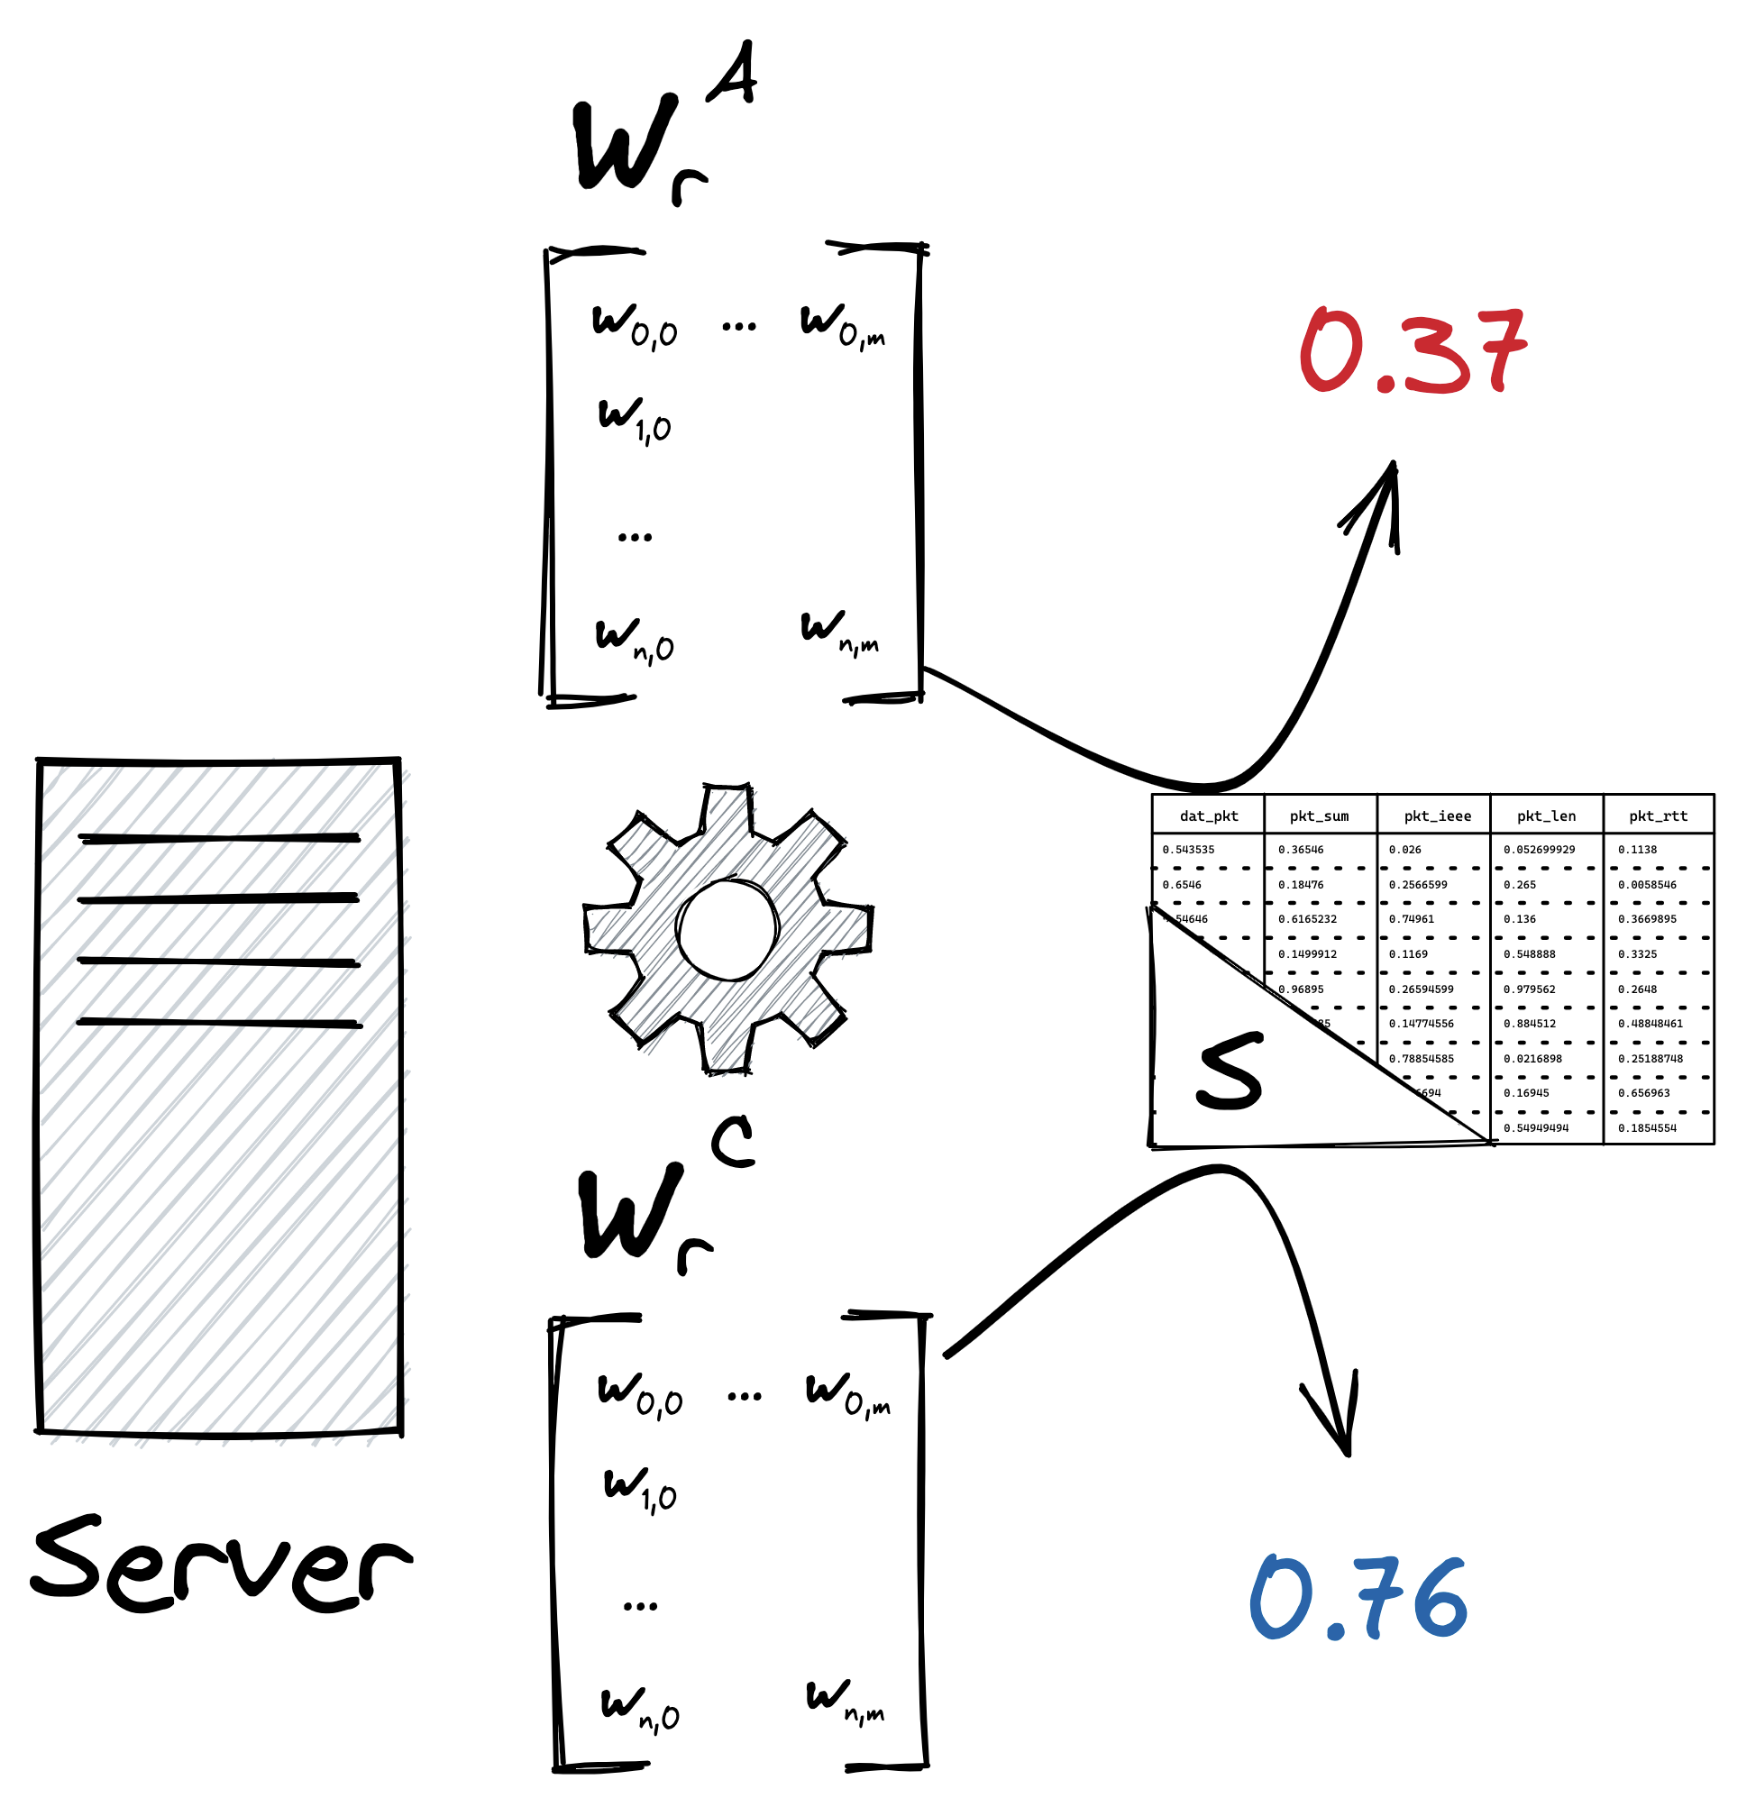
\includegraphics[height=.36\textheight]{figures/radar/server-side-eval}
      \end{figure}

      \begin{itemize}\smaller
        \item Only applicable in IID settings.
        \item Single source of truth.
      \end{itemize}
    \end{column}

    \onslide<2->{%
      \begin{column}{.33\textwidth}
        \small\centering
        \textbf{Server-side comparison}~\autocite{briggs_Federatedlearninghierarchical_2020}

        \begin{figure}
          \centering
          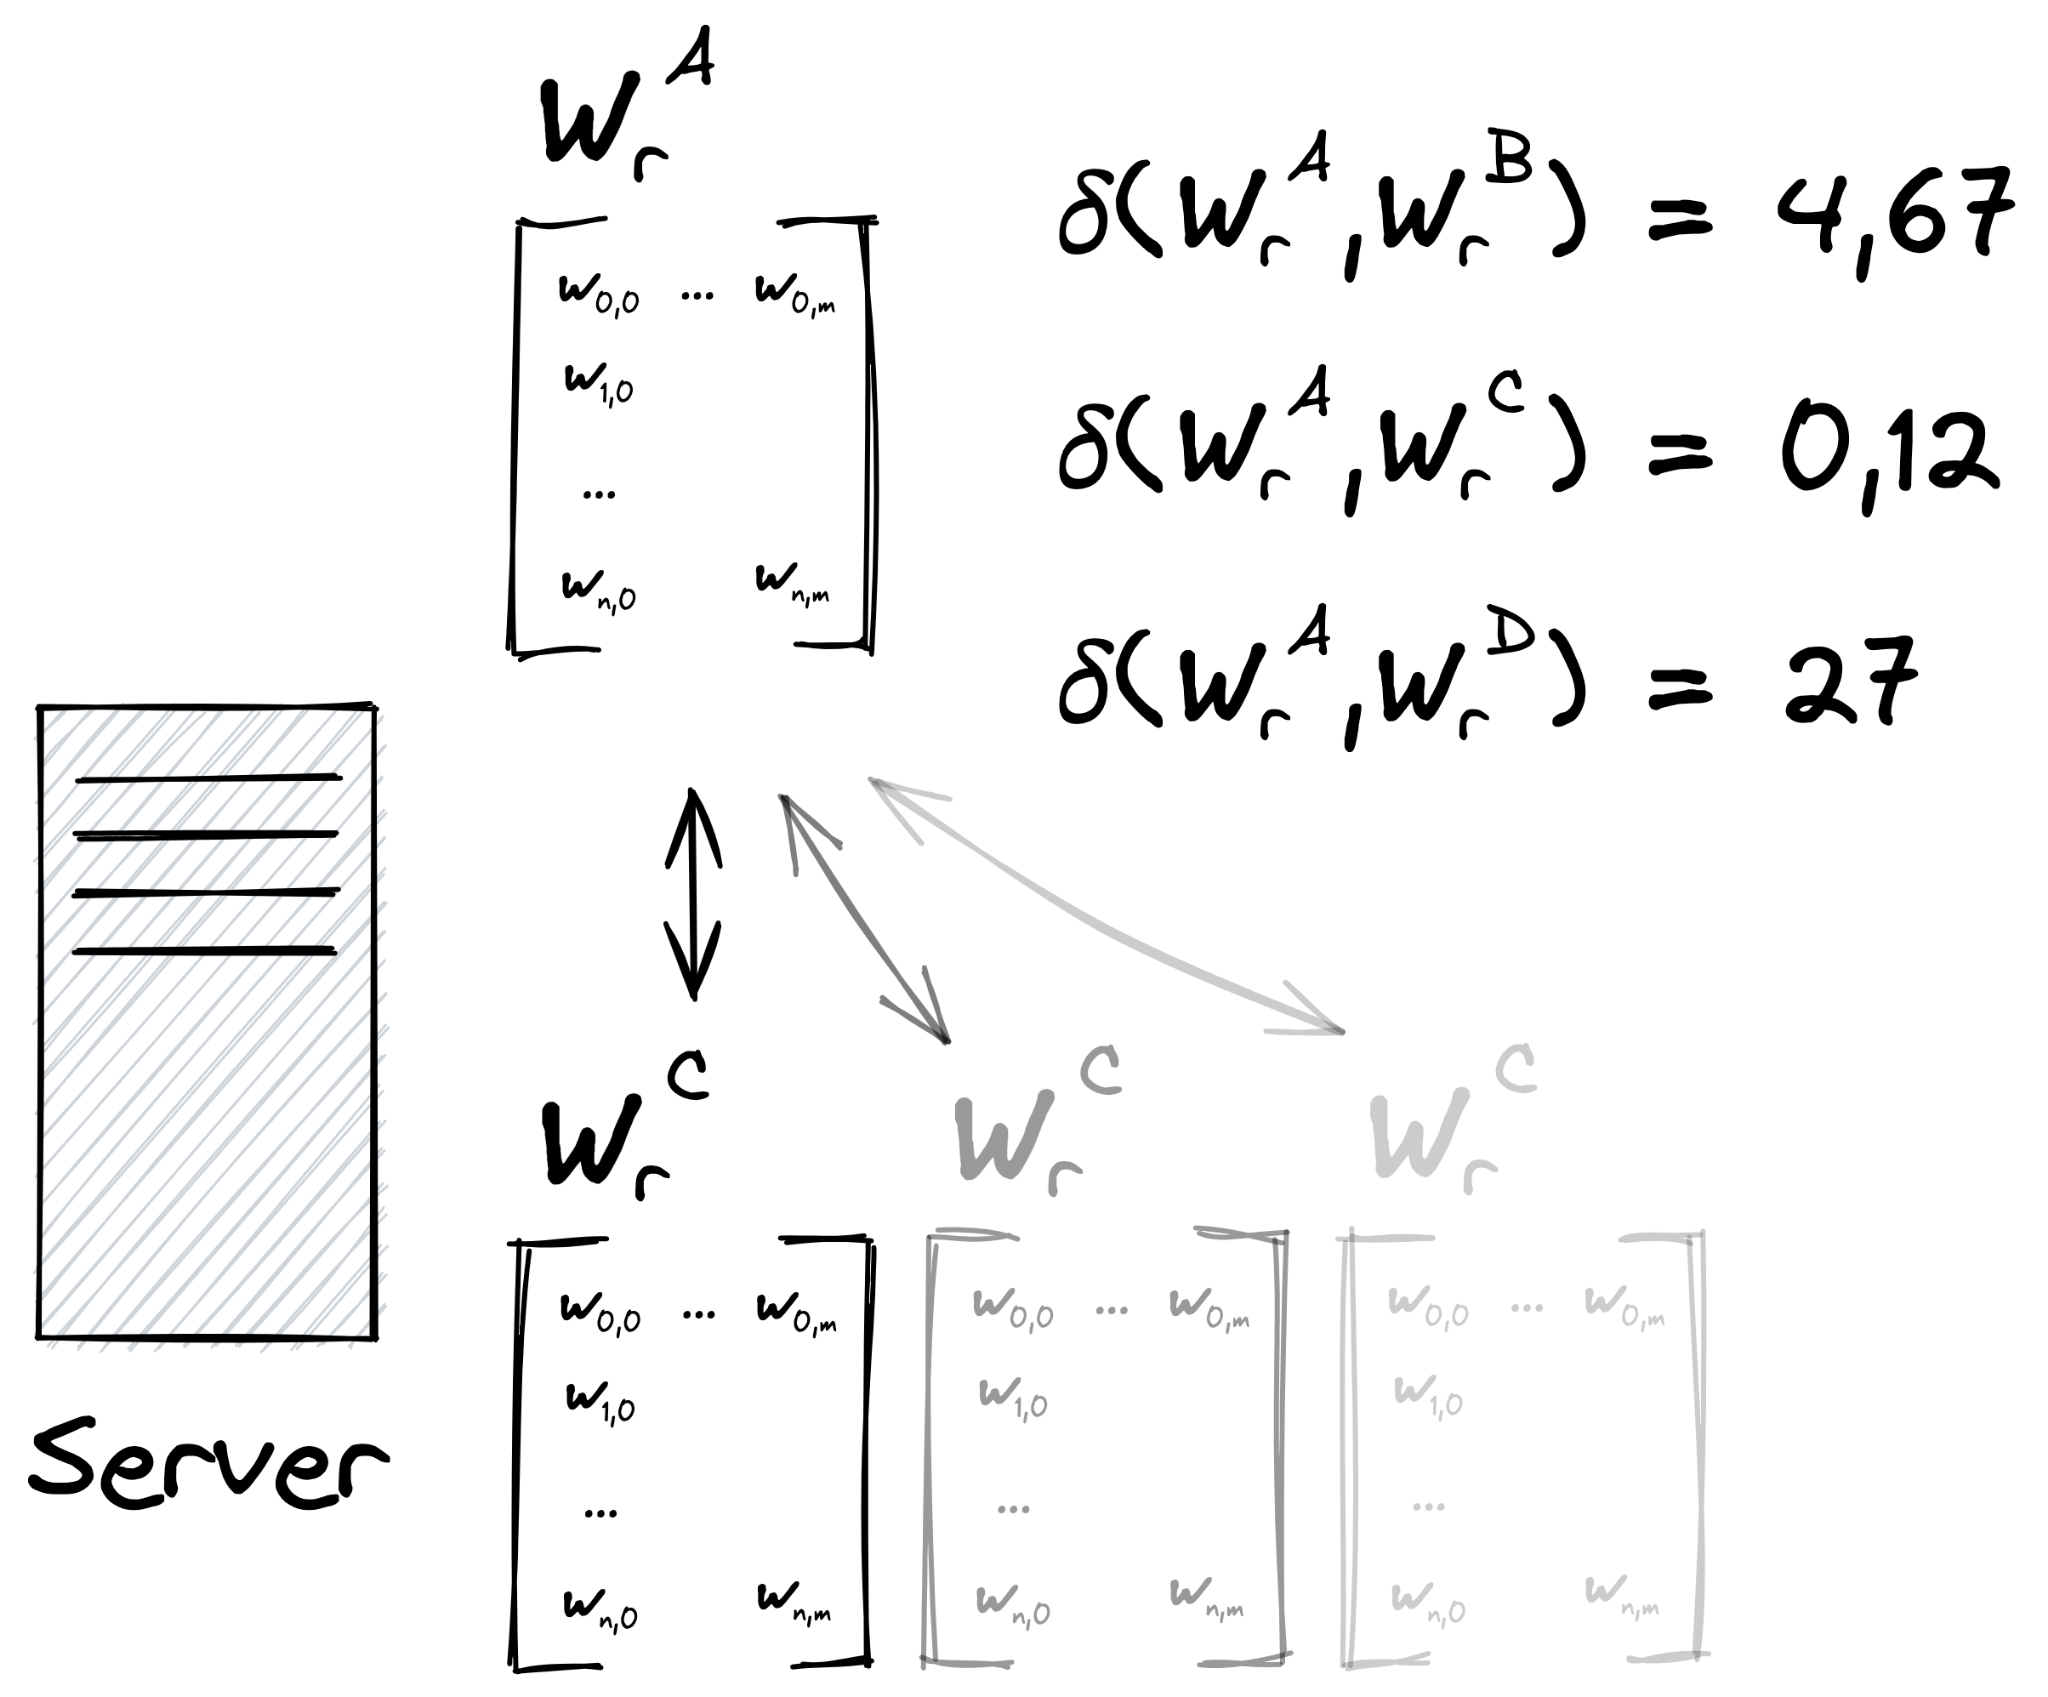
\includegraphics[height=.36\textheight]{figures/radar/server-side-comp}
        \end{figure}

        \begin{itemize}\smaller
          \item Less related to client data.
          \item More appropriate for high-dimensional data.
        \end{itemize}
      \end{column}%
    }

    \onslide<3->{%
      \begin{column}{.33\textwidth}
        \small\centering
        \textbf{Client-side evaluation}~\autocite{zhao_ShieldingCollaborativeLearning_2020}

        \begin{figure}
          \centering
          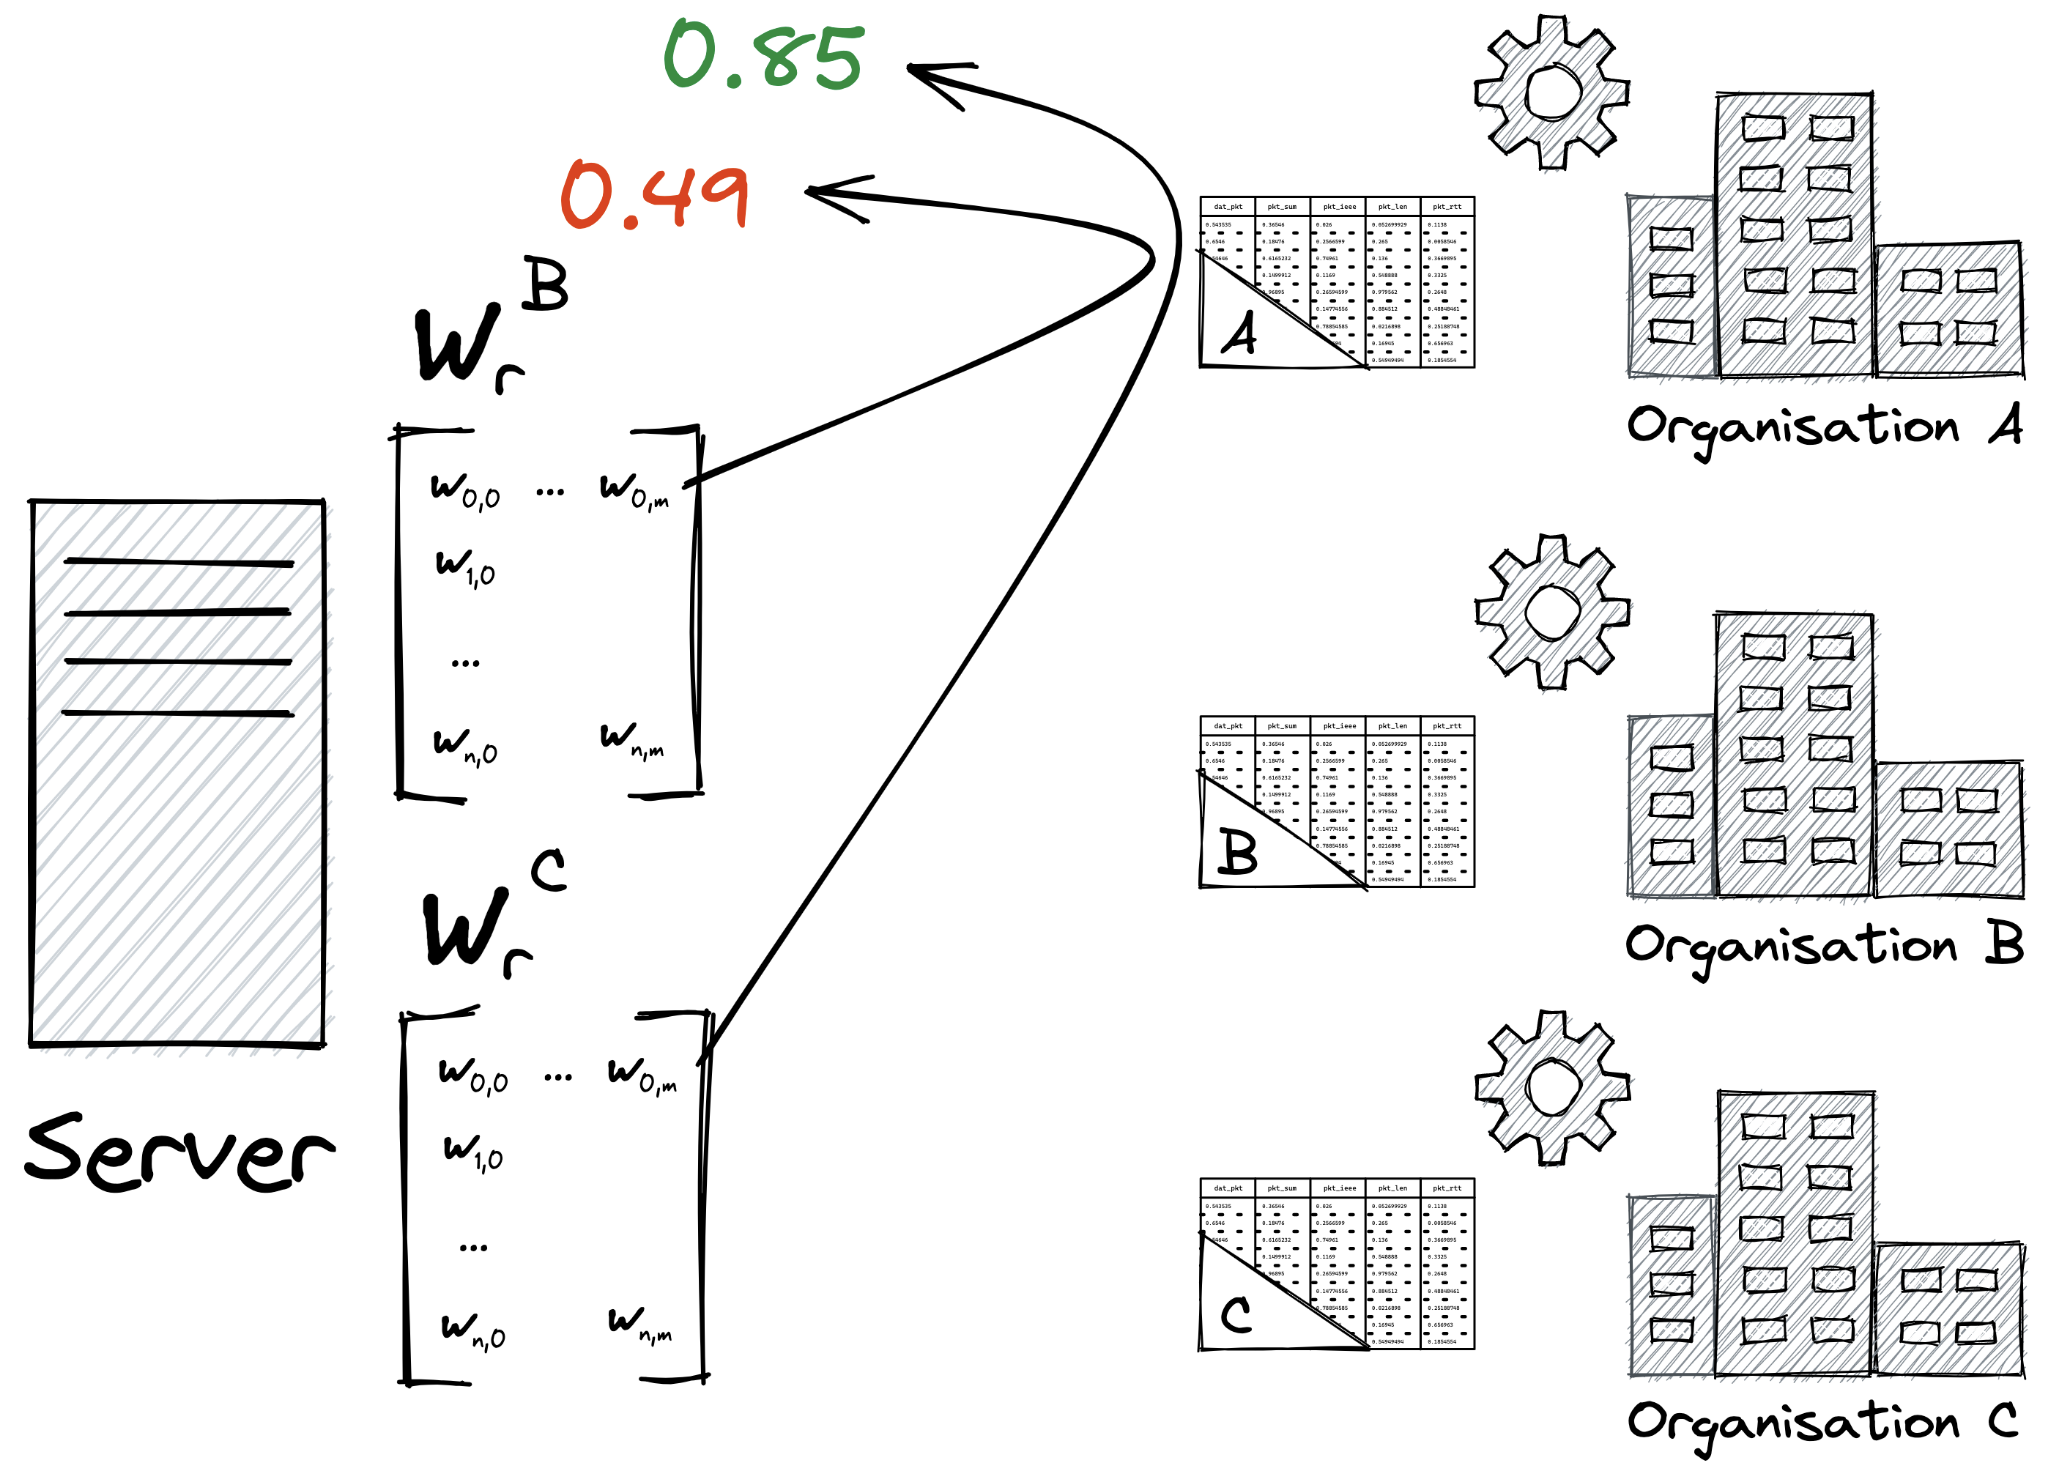
\includegraphics[height=.36\textheight]{figures/radar/client-side-eval}
        \end{figure}

        \begin{itemize}\smaller
          \item High cost in cross-device.
          \item More susceptible to badmouthing.
        \end{itemize}
      \end{column}%
    }

  \end{columns}

  \vspace{3ex}
  
  \fcitefootnote{zhou_DifferentiallyPrivateFederated_2022}
  \only<2->{\fcitefootnote{briggs_Federatedlearninghierarchical_2020}}
  \only<3->{\fcitefootnote{zhao_ShieldingCollaborativeLearning_2020}}

\end{frame}

% \begin{frame}{The RADAR Architecture}

%   \begin{figure}
%     \centering
%     \includegraphics<1>[width=.7\textwidth]{figures/radar/architecture}
%     \includegraphics<2>[width=.7\textwidth]{figures/radar/architecture-xeval}
%     \caption{The RADAR architecture.}
%   \end{figure}


% \end{frame}

\begin{frame}{Assessing Quality with Cross-Evaluation}

  \begin{columns}
    \begin{column}{.45\textwidth}
      \begin{figure}
        \centering
        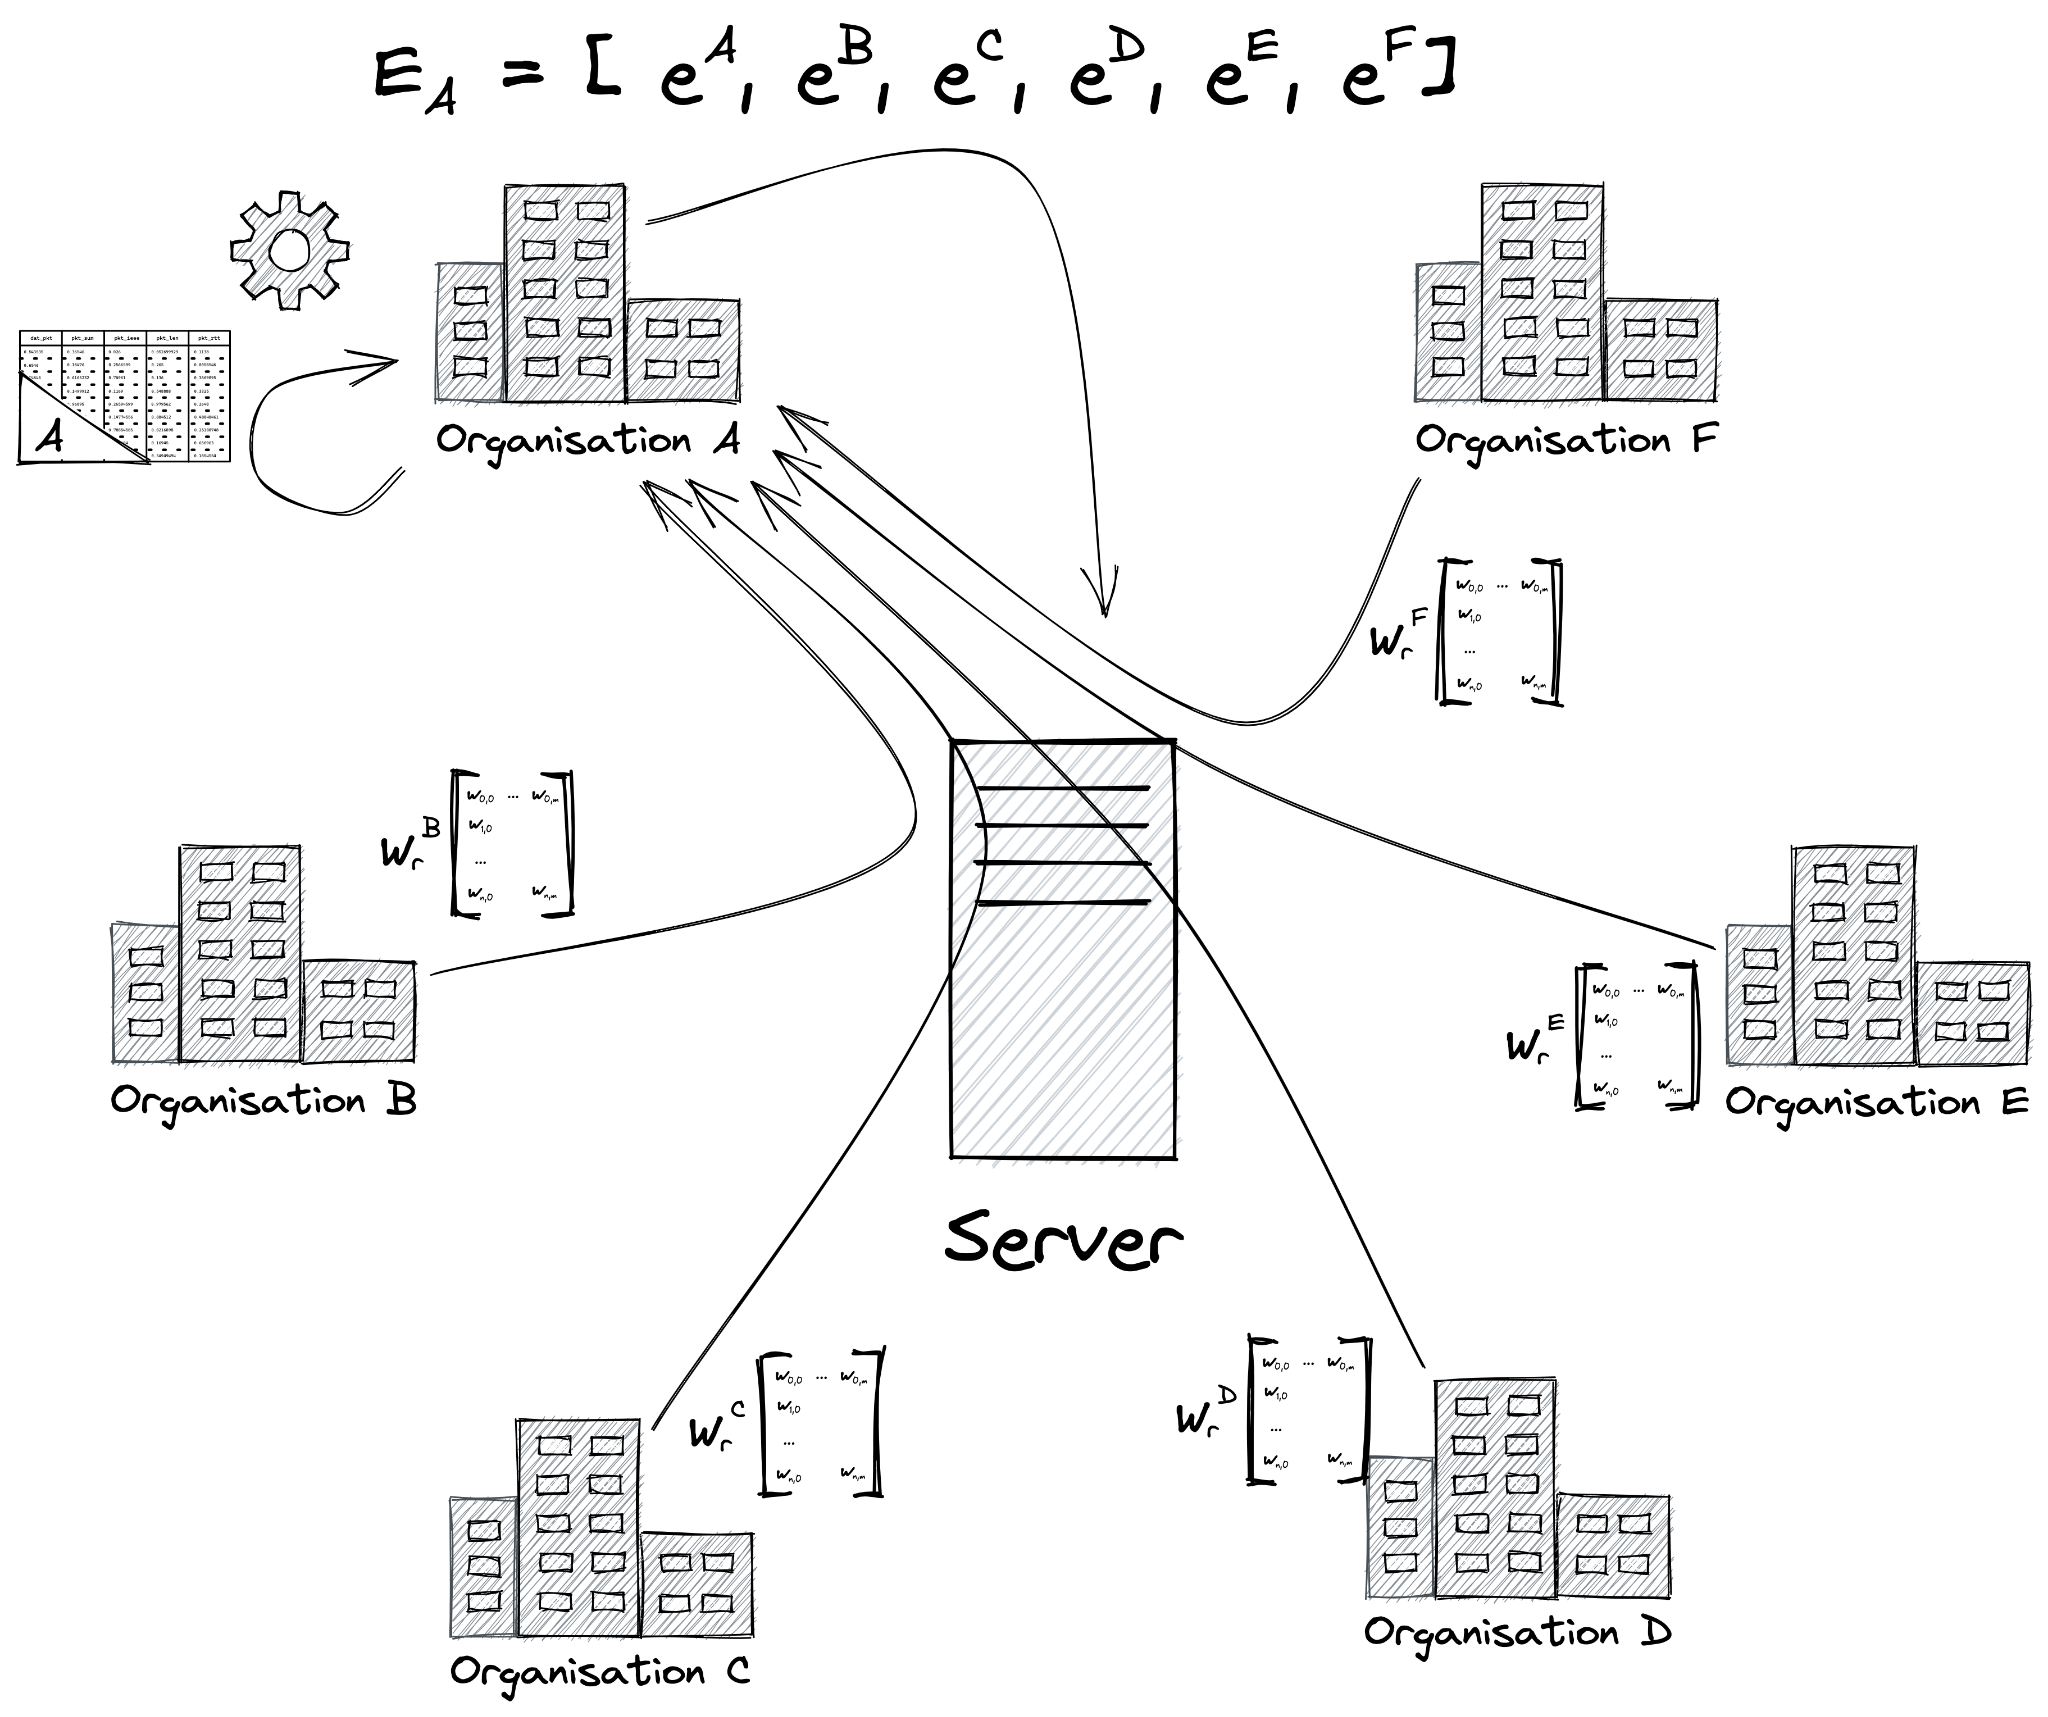
\includegraphics[width=\textwidth]{figures/radar/xeval}
      \end{figure}
    \end{column}
    
    \begin{column}{.55\textwidth}
      \small
      \setlength{\baselineskip}{0.8\baselineskip}
      \vspace{1ex}

      \textbf{Advantages}
      \begin{itemize}
        \item The central server does not need prior knowledge.
        \item Evaluates how each model fits the data (\eg, accuracy, F1 score).
        \item Exhaustive overview of the entire system at each round $r$.
      \end{itemize}

      \onslide<2->{%
        \textbf{Drawbacks}
        \begin{itemize}
          \item High communication and computation costs.
          \item Does not scale well.
          \item Shares local models to participants: less privacy-friendly.
        \end{itemize}
      }

      \onslide<3->{%
        \textbf{But\dots}
        \begin{itemize}
          \item Cross-silo use case: few clients, with reasonable computing capacity.
          \item Slow workflow: long time between rounds.
        \end{itemize}
      }   
    \end{column}

  \end{columns}

\end{frame}

\begin{frame}{Fighting Heterogeneity with Clustering}
  \begin{columns}
    \begin{column}{.55\textwidth}
      \textbf{Objective}
      \begin{itemize}
        \item Reduce heterogeneity for the aggregation.
        \item Build communities of \emph{more} homogeneous participants.
      \end{itemize}


      \onslide<2>{%
        \textbf{Clustering for FL}
        \begin{itemize}
          \item Regarding data-source:
          \begin{itemize}
            \item Gradient/model similarity.~\autocite{briggs_Federatedlearninghierarchical_2020}
            \item Cross-evaluation results.
          \end{itemize}

          \item Clustering methods:
          \begin{itemize}
            \item Dynamic \emph{split-and-merge}.~\autocite{chen_ZeroKnowledgeClustering_2021}
            \item Hierarchical clustering.~\autocite{briggs_Federatedlearninghierarchical_2020}
          \end{itemize}
        \end{itemize}
      }
      
    \end{column}
    \begin{column}{.45\textwidth}
      \begin{figure}
        \centering
        \makebox[\textwidth][c]{%
          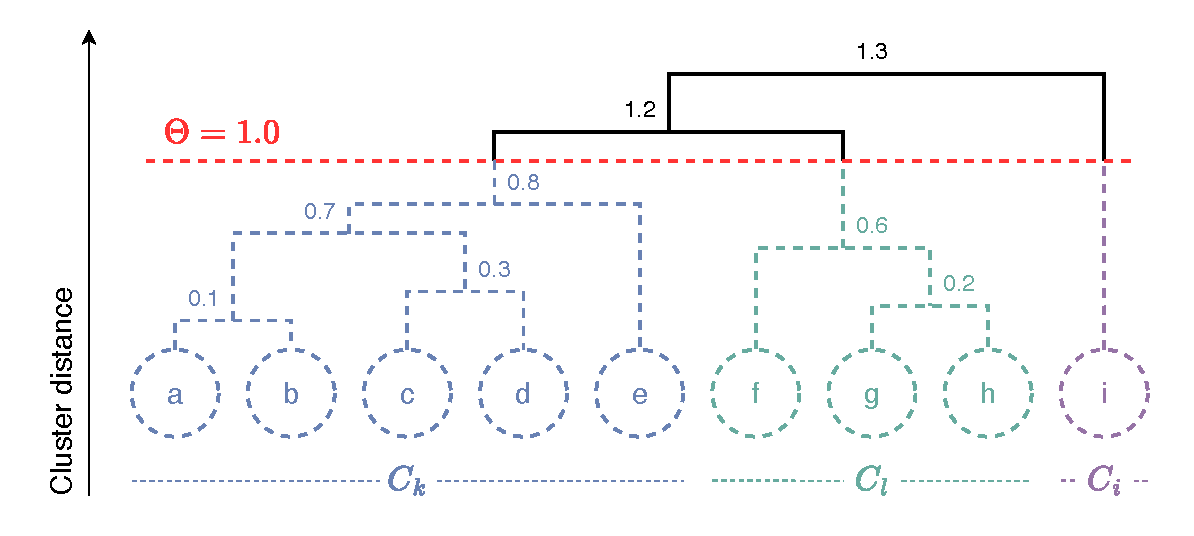
\includegraphics[width=1.2\textwidth]{figures/radar/clustering.drawio.pdf}%
        }
        %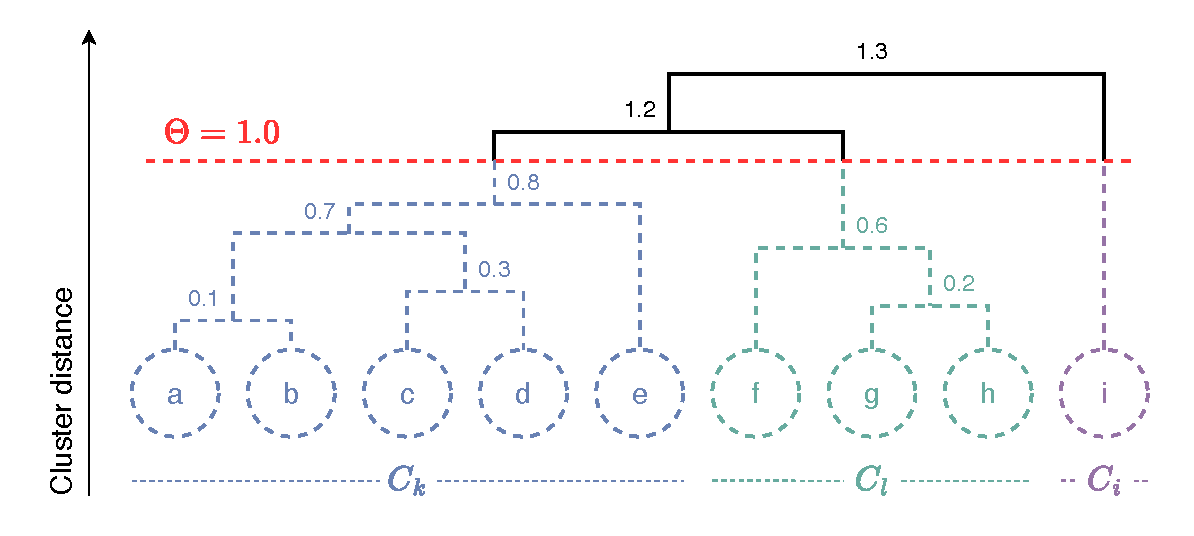
\includegraphics[width=\textwidth]{figures/radar/clustering.drawio.pdf}
        \caption{Hierarchical clustering.}
      \end{figure}
    \end{column}
  \end{columns}
  

  \only<2>{%
    \fcitefootnote{briggs_Federatedlearninghierarchical_2020}
    \fcitefootnote{chen_ZeroKnowledgeClustering_2021}
  }

\end{frame}

\begin{frame}{Reputation-aware Aggregation}

  \begin{block}{Definition: Reputation Systems\normalfont~\autocite{resnick_Reputationsystems_2000}}
    \begin{itemize}
      \item Long-lived entities that inspire an expectation of future interaction;
      \item Capture and distribution of feedback about current interactions (such information must be visible in the future); and
      \item Use of feedback to guide trust decisions.
    \end{itemize}
  \end{block}

  \onslide<2>{%
    \begin{itemize}
      \item Dirichlet distribution for local aggregation of the reputation scores.~\autocite{fung_DirichletBasedTrustManagement_2011}
      \item Votes weighted by the similarity inside each cluster.
      \item Exponential decay for potential redemption.
    \end{itemize}
  }

  \fcitefootnote{resnick_Reputationsystems_2000}
  \only<2>{%
    \fcitefootnote{fung_DirichletBasedTrustManagement_2011}
  }

\end{frame}

\begin{frame}{Experimental Setup}
  \begin{columns}
    \begin{column}{.55\textwidth}
      Similar setup as in the previous case study:
      \begin{itemize}
        \item Heterogeneous datasets, but some participants can share similarities.
        \item 4 datasets: CIC-CSE-IDS2018, UNSW-NB15, Bot-IoT, ToN\_IoT.
        \item NF-V2~\autocite{sarhan_StandardFeatureSet_2021} feature set (\ie, NetFlow V9).
      \end{itemize}
    \end{column}
    \begin{column}{.45\textwidth}
      \begin{figure}

        \includegraphics<1>[height=.5\textheight,left]{figures/radar/distribution.png}%
        \includegraphics<2>[height=.5\textheight,left]{figures/radar/distribution-attack.png}%

        \caption{Distribution of the datasets.}
      \end{figure}
    \end{column}
  \end{columns}
  \fcitefootnote{sarhan_StandardFeatureSet_2021}
\end{frame}

\begin{frame}{Results}
  \begin{table}
    \centering
    \caption{
      \emph{Effect of different attack configurations (untargeted) on all baselines.}
      \texttt{RA} is RADAR, \texttt{FG} is \texttt{FoolsGold}, \texttt{FA} is \texttt{FedAvg} (on \emph{all} participants), and \texttt{FC} is \texttt{FedAvg} ideally clustered per dataset.
    }

    \footnotesize

    \newcommand{\hl}{}
    \only<2>{\renewcommand{\hl}{\cellcolor{imta-green!30}}}


  
    \setlength\tabcolsep{1ex}
    \begin{tabularx}{.8\textwidth}{lX|rrrr|rrrr}
      \toprule % ---------------------------------
      \multicolumn{2}{c|}{\multirow{2}{*}{\textbf{Scenario}}} & \multicolumn{4}{c|}{\textbf{Mean accuracy} (\%)} & \multicolumn{4}{c}{\textbf{\gls{asr}} (\%)} \\
      & & \multicolumn{1}{c}{\texttt{RA}} & \multicolumn{1}{c}{\texttt{FG}} & \multicolumn{1}{c}{\texttt{FA}} & \multicolumn{1}{c|}{\texttt{FC}} & \multicolumn{1}{c}{\texttt{RA}} & \multicolumn{1}{c}{\texttt{FG}} & \multicolumn{1}{c}{\texttt{FA}} & \multicolumn{1}{c}{\texttt{FC}} \\
      \midrule % ---------------------------------
      % TARGETED ATTACKS
      \multicolumn{2}{l|}{\textbf{Targeted} (\texttt{100T})} & & & & & & & & \\
                  & \texttt{Benign}       & \hl 99.07 & 55.04 & 79.49 & \textbf{99.24} & \hl \textbf{0.00} &  5.17 & 5.10 &  0.09 \\
                  & \texttt{Lone}         & \hl 99.06 & 60.51 & 77.38 & \textbf{99.22} & \hl \textbf{0.00} & 93.82 & 6.73 &  0.45 \\
                  & \texttt{Collud. min.} & \hl \textbf{98.96} & 54.64 & 78.48 & 98.33 & \hl \textbf{0.00} &  2.97 & 9.99 & 53.40 \\
                  & \texttt{Collud. maj.} & \hl \textbf{98.28} & 85.10 & 79.40 & 98.22 & \hl \only<3>{\bfseries\color{red}} 73.39 & \textbf{8.10} & 17.65 & 59.36 \\
      \midrule % ---------------------------------
      % UNTARGETED ATTACKS
      \multicolumn{2}{l|}{\textbf{Untargeted} (\texttt{100U})} & & & & & & & & \\
      & \texttt{Benign}        & \hl 99.07 & 55.04 & 79.49 & \textbf{99.24} & \hl 0.09  & 0.39 & 33.30 & \textbf{0.06} \\
      & \texttt{Lone}          & \hl 98.96 & 49.56 & 78.38 & \textbf{99.22} &\hl \textbf{0.08} & 99.89 & 54.70 & 0.12 \\
      & \texttt{Collud. min.}  & \hl \textbf{98.98} & 49.67 & 72.47 & 97.69 & \hl 0.10 & \textbf{0.04} & 44.53 & 6.26 \\
      & \texttt{Collud. maj.}  & \hl \textbf{98.96} & 69.09 & 81.87 & 75.66 & \hl \textbf{0.08} & 38.98 & 59.49 & 94.36 \\          
      \bottomrule % ---------------------------------
      \small & \multicolumn{1}{c}{} & \multicolumn{4}{c}{\emph{higher is better}} & \multicolumn{4}{c}{\emph{lower is better}}
    \end{tabularx}
  \end{table}
  
\end{frame}

% \begin{frame}{Results}
%   \begin{figure}
%     \centering
%     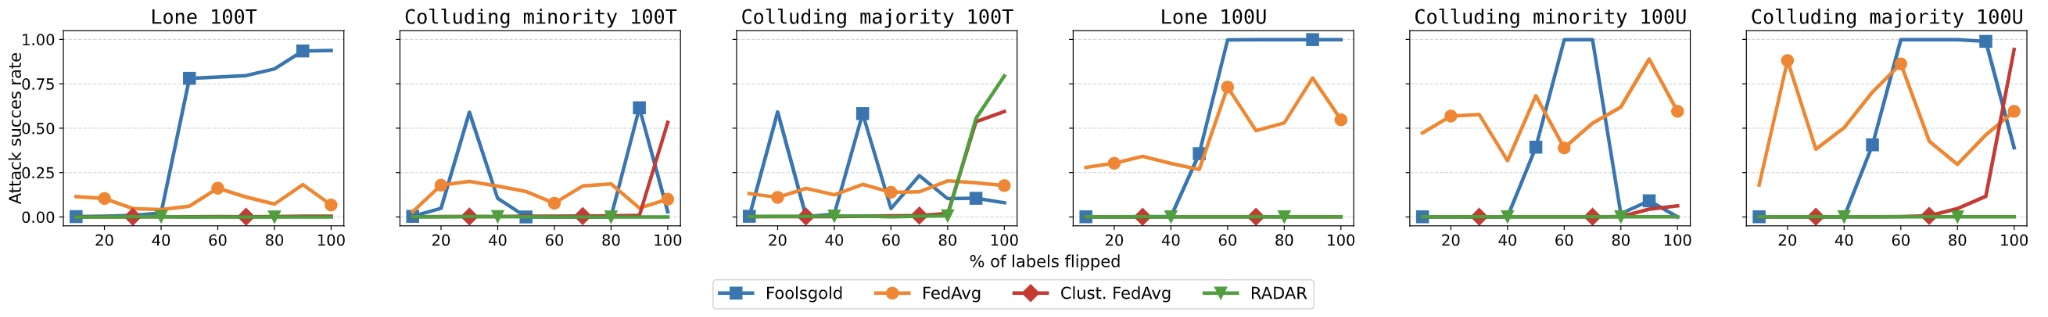
\includegraphics[width=.9\textwidth]{figures/radar/baselines.png}
%     \caption{Baseline comparison.}
%   \end{figure}
%   \begin{figure}
%     \centering
%     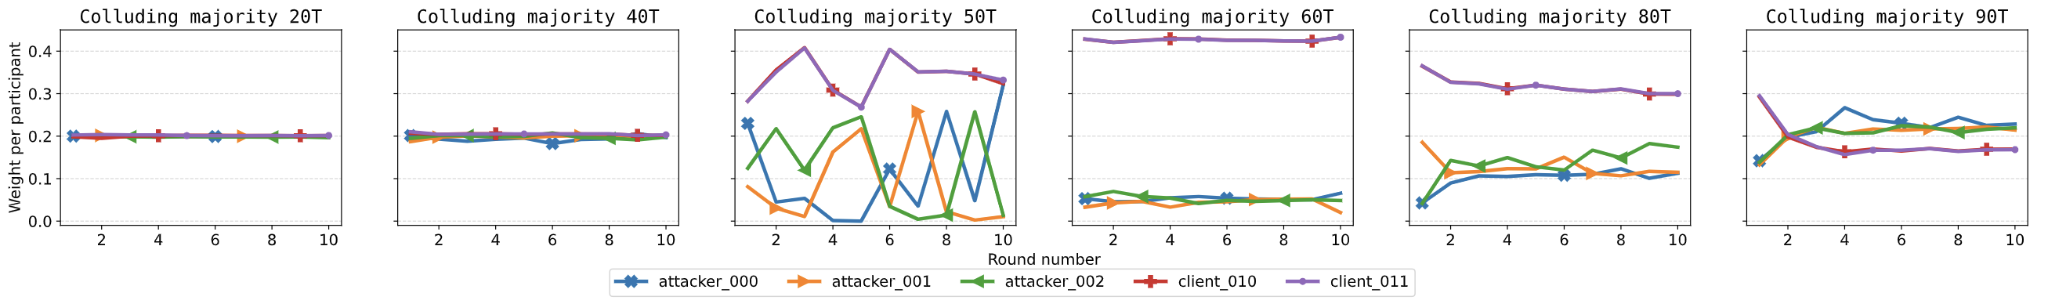
\includegraphics[width=.9\textwidth]{figures/radar/limiting-case.png}
%     \caption{RADAR's limiting scenario.}
%   \end{figure}
% \end{frame}

\begin{frame}{Takeaways}
  \textbf{The proposed framework can:}
  \begin{itemize}
    \item Accurately cluster similar participants based on cross evaluations results.
    \item Mitigate label-flipping untargeted attacks via clustering.
    \item Mitigate most label-flipping targeted attacks, including colluding attackers (up to 80\% of poisoned data).
  \end{itemize}

  \onslide<2>{%
    \textbf{Future works:}
    \begin{itemize}
      \item Remove the central server dependency.
      \item Reduce the cross-evaluation overhead to extend applicability to cross device settings.
      \item Test the approach in more realistic heterogeneous settings.
    \end{itemize}
  }
\end{frame}